\section*{Q1: Research question}
We have chosen to look at the paper “How epidemic psychology works on Twitter: evolution of responses to the COVID-19 pandemic in the U.S.“ by Aiello, L.M., Quercia, D., Zhou, K. et al. \cite{aiello2021epidemic}. We choose to look at the evolution in time of sentiment and emotion with regards to COVID-19, in the United States. 

The paper focuses on a theory called “Epidemic Psychology” by Philip Strong \cite{strong1990epidemic}, which is a sociological study of psycho-social ‘epidemics’ of fear, moralization and action that occur during major health epidemics. The authors wish to assess whether they can empirically observe these phases of emotion spreading as an epidemic through language, through the analysis of tweets, during the COVID-19 pandemic. 

Analyzing the evolution of emotion and sentiment throughout the COVID-19 pandemic through the use of tweets is a very important undertaking, as it helps inform future public health policies. Indeed, as information dissemination is extremely rapid nowadays, the spreading of fear, panic, and the amplifying misinformation, are a grave danger to public health messaging. Understanding past trends can help prevent these feelings that ultimately have a big impact on policy. Finally, we also choose to focus on the U.S. as per the paper, as the U.S. has the highest proportion of Twitter users, and because it is easier to relate evolution of emotions in time to the events of a single country.


\section*{Q2: Method choice and design}
We first select tweets whose User Location is in the U.S., and we do so by using regex-based methods of U.S. locations, as per the paper (matching to cities, states, common locations in the U.S., as well as variations on the name ‘U.S.’). This is extremely efficient and takes no more than a few seconds to run on the entire dataset, returning approximately 103K U.S.-based tweets from a preprocessed dataset of 382K tweets. 

We then run the VADER sentiment analysis on this subset, aggregate the scores of tweets over the course of a week, normalize these figures by the number of total tweets that week, and plot it. The result is shown in \cref{fig:p3-fig9}. We do not provide a code snippet for VADER as it is almost identical to the one in Part 2. 

For completeness’ sake, we compare with the ground truth labels aggregated and plotted in a similar fashion (the positive labels and absolute values of negative labels are averaged over the course of a week). While this is not sentiment analysis, it provides a comprehensive view of the dataset. This is shown in \cref{fig:p3-fig10}. For completeness, we also plot the number of tweets per week in \cref{fig:p3-fig11}, as this puts our findings in context, and shows the evolution of the interest in the topic of COVID-19.

In \cref{listing:p3-listing3}, we show how we sort the time stamps, and aggregate any column into weekly counts and normalize by the number of tweets.

\begin{listing*}
\caption{Timestamp sorting, resampling weekly, normalizing by number of tweets.}
\begin{minted}{python}
# end up with 103k tweets we are sure are in the US
df_tweets_US = df_tweets_US.set_index('Timestamp').sort_values(by='Timestamp', ascending=True)
df_tweets_US.index = df_tweets_US.index.astype('datetime64[ns]')
df_tweets_US[['pos_sent', 'neg_sent']] = df_tweets_US[['pos_sent', 'neg_sent']].astype('int')
df_tweets_US['neg_sent'] = df_tweets_US['neg_sent'].abs()
df_tweets_US = df_tweets_US.rename(columns={'US_or_not': 'TweetCount'})

df_US_weekly = df_tweets_US.resample('W').sum() # sum of positive and negative
df_US_weekly['avg_pos'] = df_US_weekly['pos_sent']/df_US_weekly['TweetCount']
df_US_weekly['avg_neg'] = df_US_weekly['neg_sent']/df_US_weekly['TweetCount']
\end{minted}
\label{listing:p3-listing3}
\end{listing*}

Just like in the paper, we then choose a lexicon, the NCR lexicon (also called Emolex), which categorizes words into 8 emotions (or none): Anger, Anticipation, Disgust, Fear, Joy, Sadness, Surprise, and Trust. For every token in the preprocessed, tokenized, stemmed tweets, we match to the lexicon and count the number of occurrences of each emotion for all tweets. This process is shown in \cref{listing:p3-listing4}. As above, we then aggregate our findings over the course of the week, normalize these counts by the number of tweets of that week, and plot our findings as a heatmap.

\begin{listing*}
\caption{Emotion analysis on our dataset using the NCR/Emolex lexicon, then resampling weekly and normalization of counts by number of weekly tweets as usual.}
\begin{minted}{python}
# Importing the data from the NCR lexicon
ncr = pd.read_csv('NCR-lexicon.csv', sep =';')
emotions = ['Anger', 'Anticipation','Disgust','Fear', 'Joy','Sadness', 'Surprise', 'Trust']
stemmer = SnowballStemmer("english")
df_emotions = pd.DataFrame(0, index=df_tweets_US.index, columns=emotions)

for i, row in df_tweets_US.iterrows(): # for each tweet
   tweet = row['unigram']
   for word in tweet: # for each token in tweet
       word_stemmed = stemmer.stem(word) # stem token
       # check if the word is in NRC
       result = ncr[ncr.English == word_stemmed]
       # we have a match
       if not result.empty:
           # update the tweet-emotions counts
           for idx, emotion in enumerate(emotions):
               df_emotions.loc[i, emotion] += result[emotion].values
df_emotions_weekly = df_emotions.resample('W').sum() # sum of positive and negative
df_emotions_weekly = df_emotions_weekly[['Anger','Anticipation', 'Disgust', 'Fear', 'Joy', 'Sadness', 'Surprise', 'Trust']].div(df_US_weekly.TweetCount, axis=0)
\end{minted}
\label{listing:p3-listing4}
\end{listing*}

We then perform change point detection as per the paper, which we plot over this weekly emotion heatmap. The change points and the emotions heatmap are shown in \cref{fig:p3-fig12}, and the code snippet is shown in \cref{listing:p3-listing5}.
As this is an unsupervised task, we do not propose any quantitative performance metrics to measure the success of our approach. However, we can qualitatively assess our methods, by comparing changes in the plots to certain events occurring in the U.S. at that time that relate to the COVID-19 pandemic.

\begin{listing*}
\caption{Change point detection on weekly emotion heatmap.}
\begin{minted}{python}
from scipy.signal import find_peaks
grouped = df_emotions.groupby(pd.Grouper(freq='W'))

gradients_em = pd.DataFrame(grouped.apply(lambda x: np.mean(np.square(np.gradient(x, axis=0)), axis=0)), columns=['Values'])['Values'].apply(pd.Series)
gradients = pd.DataFrame(grouped.apply(lambda x: np.mean(np.square(np.gradient(x, axis=0)))))
change_points, _ = find_peaks(gradients[0], height=np.mean(gradients[0]) + 1.5 * np.std(gradients[0]))
print('Global change points detected at:', change_points)

# plot as heatmap as there are 8 values for each week
fig, ax = plt.subplots(figsize=(20,7))
ax = sns.heatmap(df_emotions_weekly.T, ax=ax, cmap='Blues')
ax.set_xticklabels(df_emotions_weekly.index.strftime('%d-%m-%Y'))
plt.xticks(rotation=45)
ax.vlines(change_points, *ax.get_ylim(), color='red', linewidth=7)

for cnt, i in enumerate(gradients_em.columns):
   change_points, _ = find_peaks(gradients_em[i], height=np.mean(gradients_em[i]) + 1.5 * np.std(gradients_em[i]))
   print('Local change points for emotion', emotions[i], 'detected at:', change_points)
   ax.vlines(change_points, cnt+1, cnt, color='black', linewidth=4)

plt.show()
\end{minted}
\label{listing:p3-listing5}
\end{listing*}


\section*{Q3: Results \& Analysis}
As stated above, we summarize our findings through the figures shown below.

\begin{figure}
    \centering
    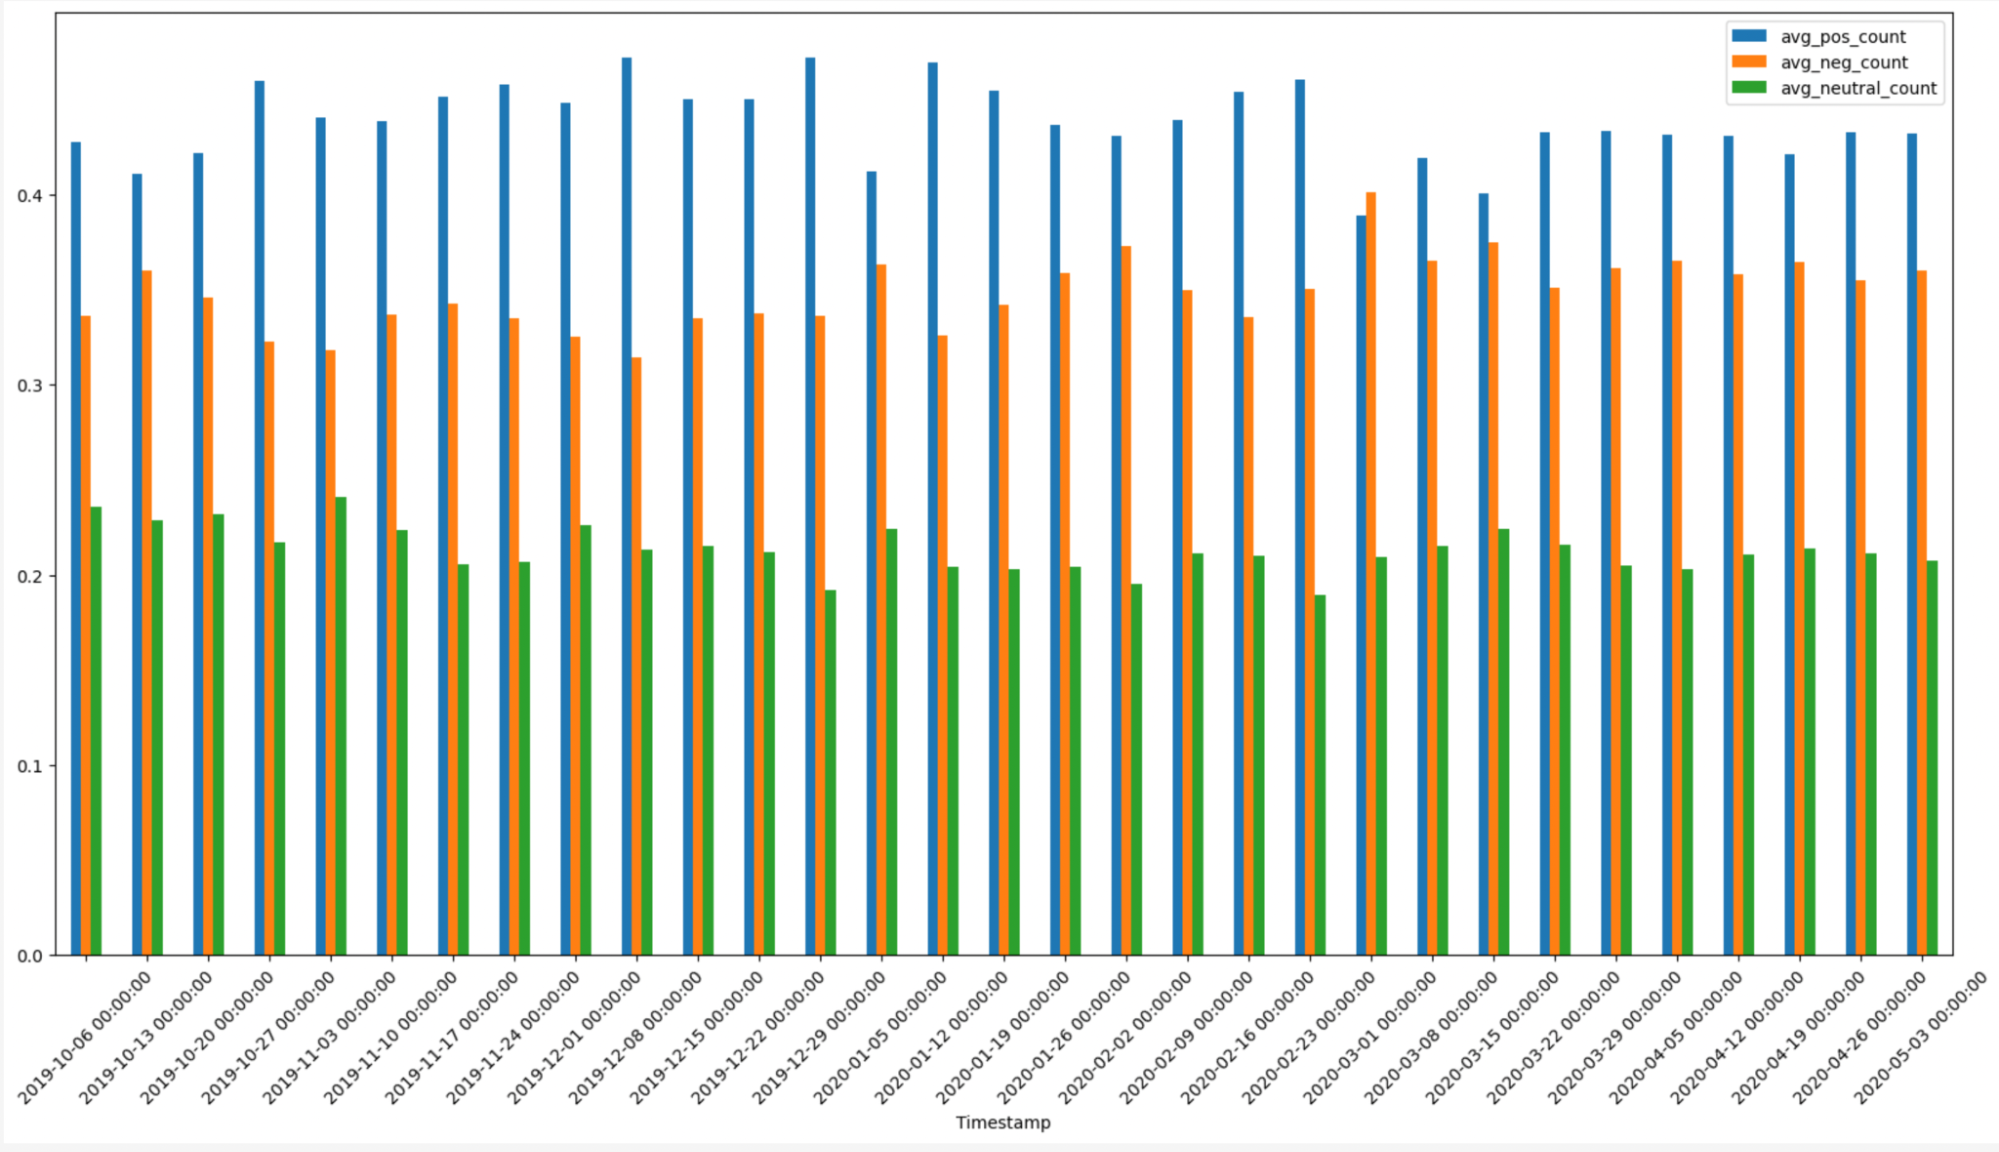
\includegraphics[width=0.9\textwidth]{images/p3_fig9.png}
    \caption{VADER sentiment scores aggregated weekly and normalized by the number of tweets that week.}
    \label{fig:p3-fig9}
\end{figure}
\begin{figure}
    \centering
    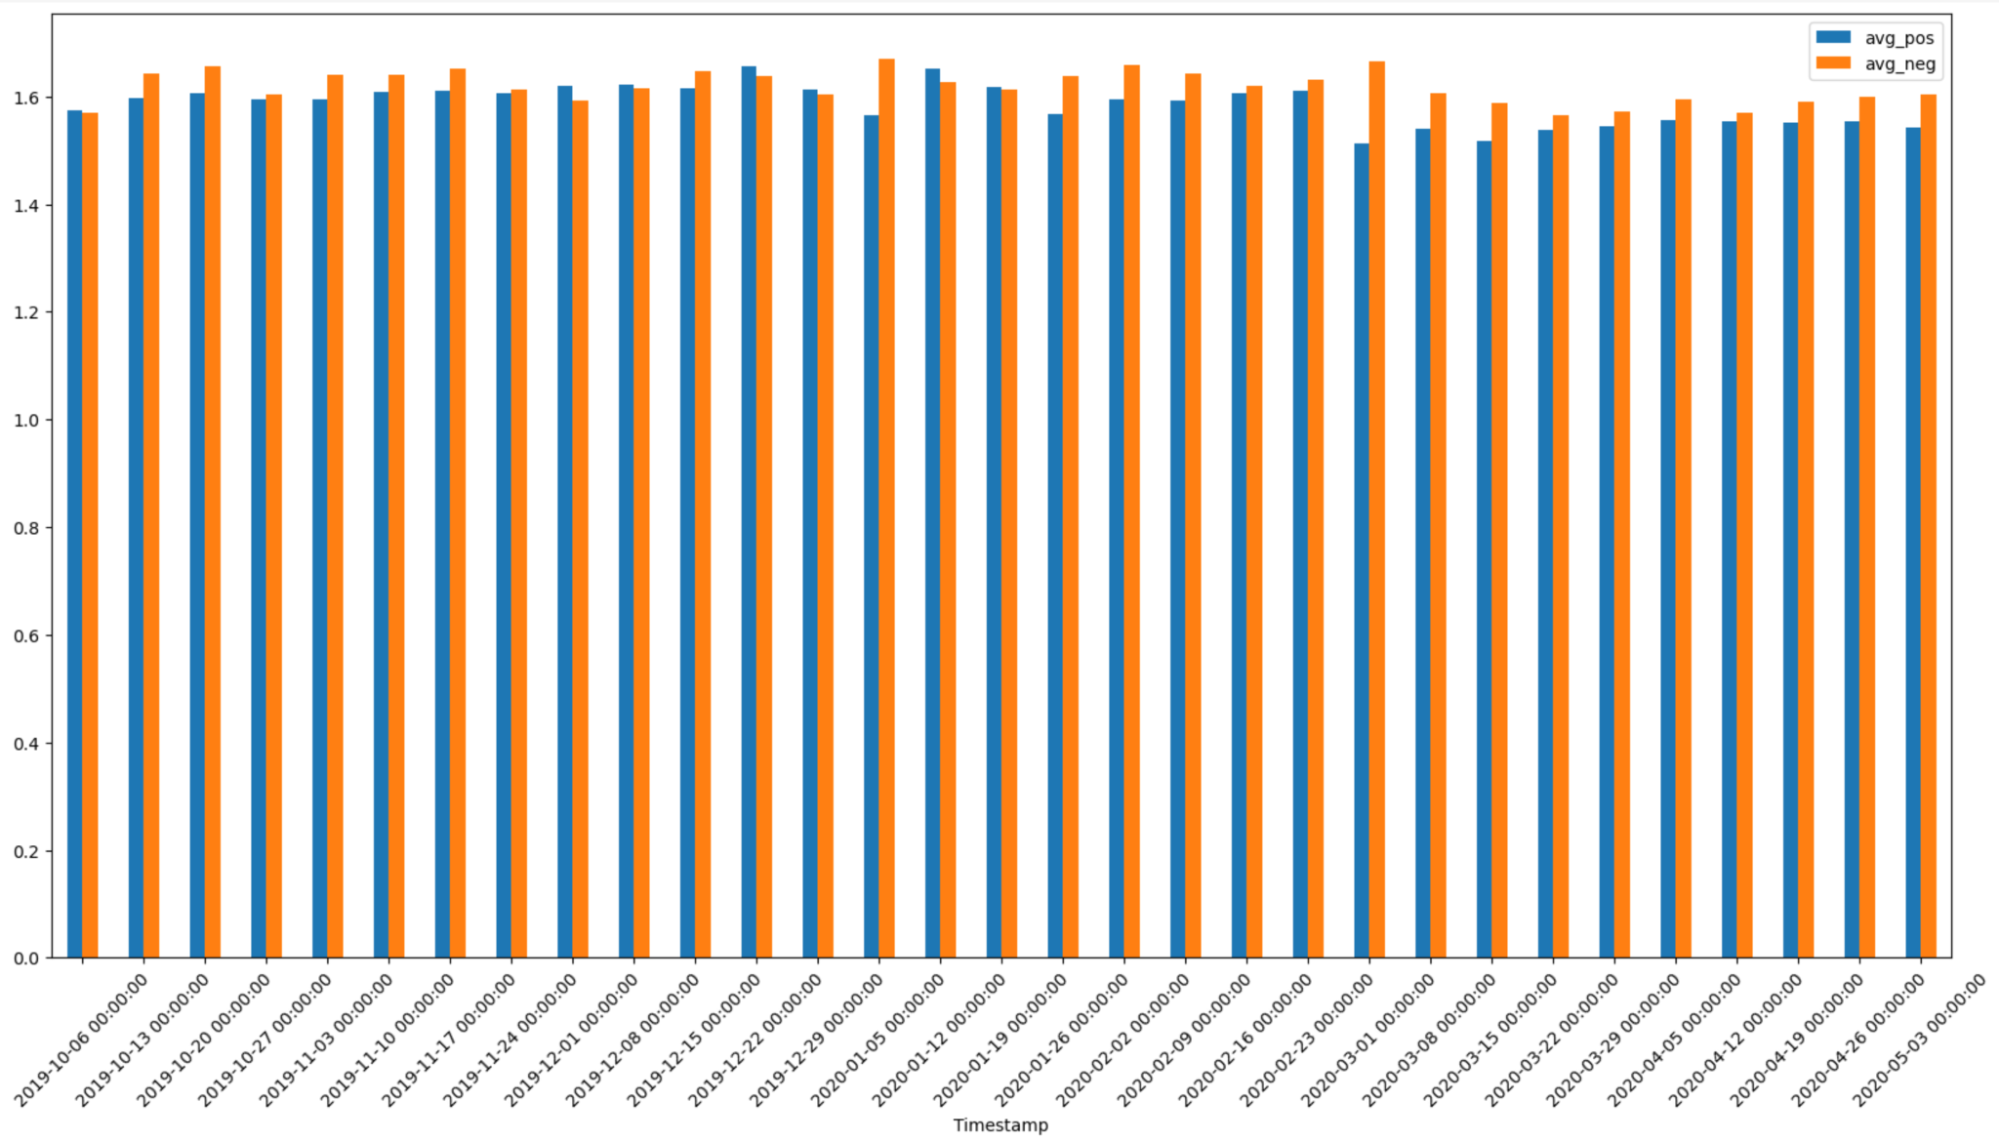
\includegraphics[width=0.9\textwidth]{images/p3_fig10.png}
    \caption{Ground truth labels averaged over each week (the absolute values of the negative labels are taken).}
    \label{fig:p3-fig10}
\end{figure}

Looking at the VADER analysis in \cref{fig:p3-fig9}, we observe that while the normalized positive and negative sentiments fluctuate in time, we very clearly observe a clear difference in the week 23/02/2020. Every week always has always had a higher proportion of positive tweets than negative, except this week. After this week, every subsequent week has had a fewer proportion of positive tweets. This is also observed in the ground truth labels in \cref{fig:p3-fig10}, albeit less notably.

\begin{figure}
    \centering
    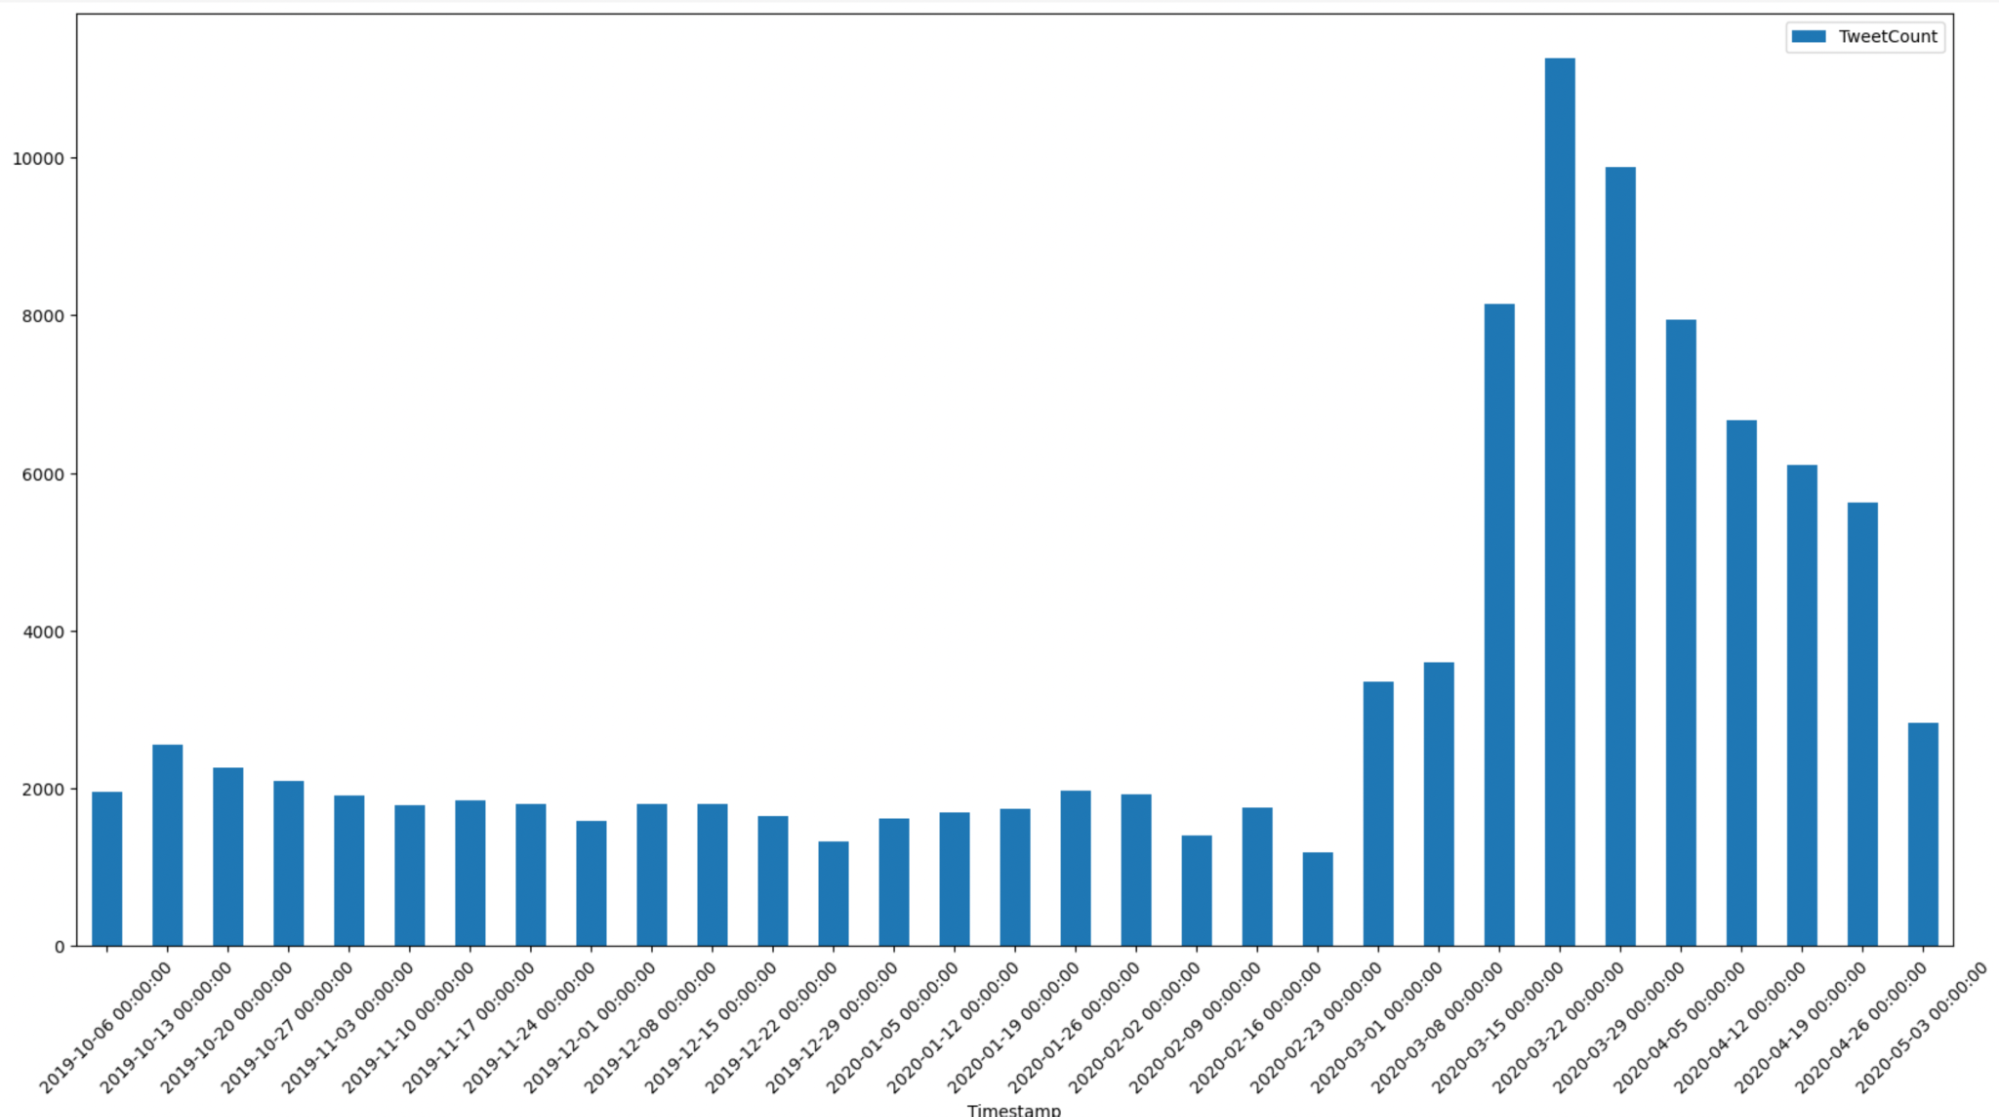
\includegraphics[width=0.9\textwidth]{images/p3_fig11.png}
    \caption{Number of tweets per week pertaining to COVID-19 in the US (subset of given dataset).}
    \label{fig:p3-fig11}
\end{figure}
\begin{figure}
    \centering
    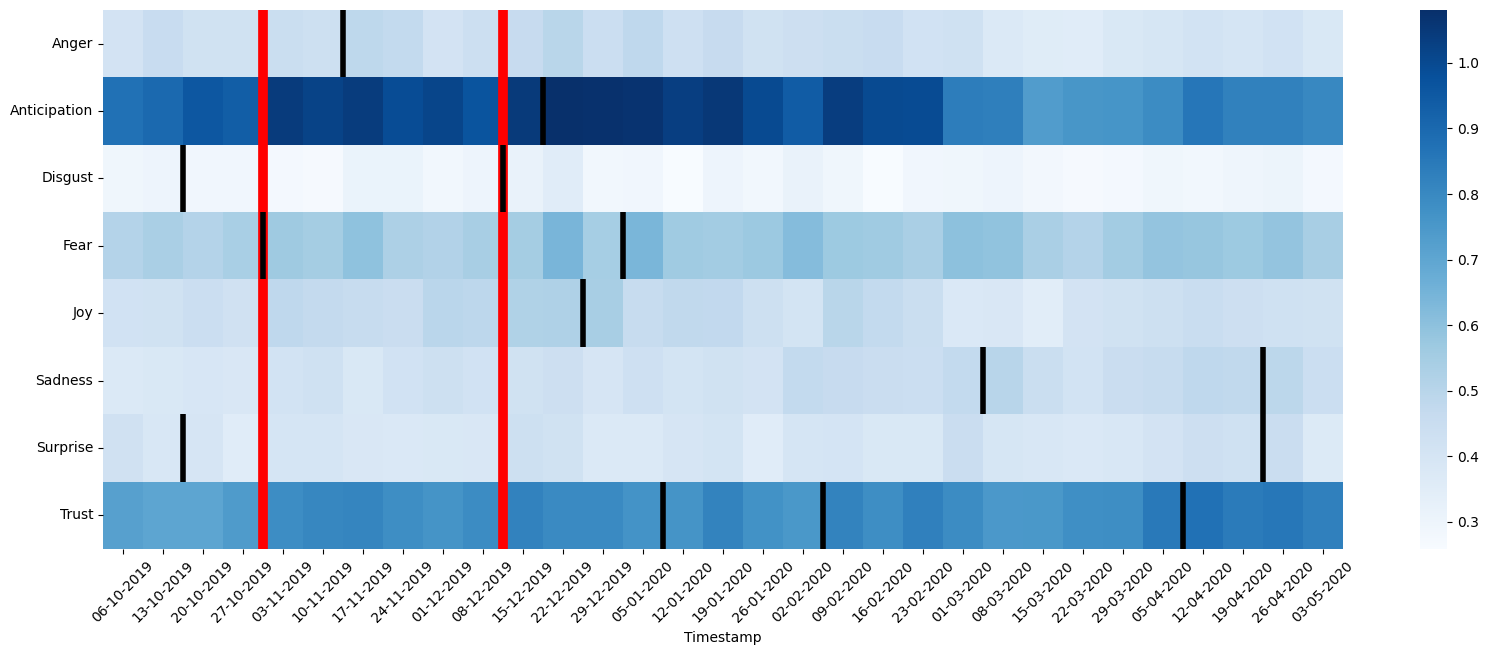
\includegraphics[width=0.9\textwidth]{images/p3_fig12.png}
    \caption{Heatmap of emotion analysis, aggregated weekly, normalized over the number of tweets every week. Change points are overlaid on this heatmap (red: global change point, black: local change point).}
    \label{fig:p3-fig12}
\end{figure}

The heatmap shown in \cref{fig:p3-fig12} shows that there is a sharp drop in Anticipation after, and including, the week of 23/02/2020. This change is also observed, albeit less markedly, in Fear (increase), Joy (decrease) and Sadness (increase), which agrees with our observations from the VADER plot. Since the week of 23/02/2020 approximately corresponds to when COVID-19 took over news coverage, with the constant publication of new COVID cases spreading across the country, we qualitatively judge our methods to be successful as we can see a marked change across the heatmap (Emolex) and our sentiment analysis (VADER) at approximately the same time. This is thus when the public truly became aware of the threat of the virus.

Using change point detection, we can confirm the change in Sadness at the start of the pandemic, and additionally see a peak in joy right around Christmas week, with Fear apparently at its height around New Year.
We thus see that emotion analysis through a lexicon is a powerful tool to understand public perception of a major health crisis, as we can clearly see changes in sentiment and emotion occurring at approximately the times which correspond to international and nationwide events.


\section*{Q4: Comparison to literature}
As shown above, we do see a change in emotions and sentiments corresponding to major events. However, it is difficult to make an analysis of actual phases as in the paper -- the authors found phases of refusal, anger and acceptance. The difficulty that we face in order to replicate that in our case, is due to the fact that our dataset ends much earlier (theirs ends at the end of 2020, whereas ours ends in May 2020, a mere two months after discussions on the pandemic were widespread across the U.S.), and due to the fact that we have a lot less tweets (they have 122M, while we have 103K). It is thus not possible, due to the dataset, to carry out an analysis of phases or ‘epidemic psychology’ and seeing how they coincide with contagion waves.


\section*{Q5: Discussion}
The authors have constructed their own methodology consisting of their own lexicon based on four lexicons, while we used a readily available one, the NCR/Emolex lexicon. This is due to the fact that we are running a study on a much smaller scale. We also implemented change-points just as in the paper, however, we added VADER sentiment analysis in order to understand the correlations between the changes in emotions and whether they are positive or negative.

The smaller scale of this study and the dataset limitations thus mean that it is difficult to compare our work to the paper’s, however, our work shows that, even with severe limitations, it is possible to see significant changes in emotions and sentiment that coincide with major events across a country.

The advantage of our methods are that they are extremely simple and efficient, however this is also a disadvantage compared to the paper, as our techniques are not as extensive and fine-tuned as those of the authors.

\section*{Q6: Summary \& Conclusion}
Through the use of unsupervised sentiment analysis techniques, such as VADER, emotion lexicon-matching and change point detection, we are able to detect significant changes in emotion and sentiment in completely unstructured and brief social media texts. This is a significant finding, even as the dataset used was small and significantly shorter than the actual duration of the pandemic, as it indicates that unsupervised sentiment analysis techniques are powerful enough to actually detect human emotion in the absence of labels. Our simple methodology is hence a success, as we can demonstrate that these techniques are valuable to analyze public perception at a very large scale, and can help inform public health policy.

